\section{Introdução}

\epigraph{\justifying A capacidade de reduzir tudo a leis fundamentais simples
não implica na capacidade de partir destas e reconstruir o universo. A hipótese
construcionista se desfaz quando confrontada com o par de dificuldades de escala
e complexidade. A cada camada de complexidade surgem propriedades totalmente
novas. Psicologia não é uma aplicação da biologia, e muito menos a biologia uma
aplicação da química. Agora vemos que o todo torna-se não algo além, mas algo
completamente diferente da soma de suas partes.}{\emph{Philip W. Anderson}, More
is Different: Broken Symmetry and the Nature of the Hierarchical Structure of
Science (1972)}

\noindent A termodinâmica é área da física que lida com \emph{emergência}, ou
seja, propriedades, leis ou fenômenos que ocorrem em escalas macroscópicas -
quando o número de constituintes torna-se grande - que não surgem naturalmente
na escala microscópica - na dinâmica fundamental dos constituintes, apesar de
por definição o sistema macroscópico podendo ser visto como um grande conjunto
de sistemas microscópicos sujeitos a tais leis dinâmicas.

\subsection{Escala}

Com o objetivo de capturar o que acontece quando nossos sistemas tornam-se
grandes e macroscópicos, introduzimos a noção de \emph{transformação de escala}
para os nossos sistemas de interesse, onde caracterizamos o comportamento de uma
grandeza física $X$ quando alteramos o tamanho por um fator $\lambda$ com uma 
\emph{lei de escala} dada por uma função positiva e monotônica $f$. Escrevemos
$$X\sim f(\lambda)$$
quando $X$ torna-se $f(\lambda)X$ sob uma transformação de escala. 

Dois tipos de lei de escala são especiais o suficiente para receberem nomes. Uma
grandeza é dita \emph{extensiva} quando sua lei de escala é proporcional, $X\sim
\lambda$, normalmente denotada por letras maiúsculas. Uma grandeza é dita \emph{
intensiva} quando sua lei de escala é constante, $y\sim1$, normalmente denotada
por letras minúsculas.

Note que a noção de escala é ambígua: poderiamos reformular todas as leis de
escala para usar $\lambda^2$, $1/\lambda$, $2^\lambda$ ou qualquer outra função
monotônica como parâmetro, e como consequência a noção de extensividade como
aqui apresentada está sujeita a essa mesma ambiguidade. Nas situações em que
essa confusão pode se manifestar, costuma-se utilizar diretamente alguma
grandeza de referência $\Lambda$ ao invés do parâmetro de escala no enunciado
dessas leis, onde fica implícita a extensividade de $\Lambda$, e portanto a de
qualquer grandeza para qual dizemos que $X\sim\Lambda$. De forma geral,
$\Lambda$ assim como as equações que regem as relações entre grandezas vão ser
tratadas como propriedades fixas do sistema em questão, enquanto as outras
grandezas serão tomadas como sujeitas a mudança, chamadas \emph{variáveis de
estado}.

\subsection{Calor}

A medida que um sistema torna-se complexo vamos perdendo a capacidade de
descrever e controlar precisamente as interações entre seus constituintes. Cada
um destes move-se de acordo com a dinâmica microscópica exercendo e estando
sujeito a forças dos outros de forma que os detalhes vão muito além da
especificidade de qualquer preparação experimental. Este movimento errático
dentro de um sistema físico é justamente o que nos permite caracterizar suas
propriedades através de leis de escala, uma vez que é responsavel por
redistribuir bolsões de certas grandezas ao longo de um sistema todo.

Quando lidamos especificamente com a energia, o efeito resultante destas várias
pequenas transferências de trabalho irregulares, o \emph{calor}, ainda que
sujeito à lei da conservação de energia, comporta-se de forma distinta do
trabalho que estamos acostumados na mecânica, e deve ser caracterizado como tal.
O calor é energia térmica em trânsito. Quando dois sistemas estão em uma
configuração que possibilita a troca de calor entre eles, são ditos em \emph{
contato térmico}. Um meio que permite a transferência de calor entre sistemas é
dito \emph{diatérmico}. Do contrário, um que não a permite, é dito \emph{
isolante}.

Da mesma maneira que o movimento irregular dos constituintes gera uma
redistribuição de grandezas dentro de um próprio sistema, ela pode também
acarretar algo semelhante entre sistemas, afinal a fronteira que separa um
sistema do outro quando estes são interagentes é uma construção teórica. Quando
dois sistemas encontram-se em uma situação onde a troca de calor entre eles é
possível, porém não ocorre de forma apreciável, são ditos em \emph{equilíbrio
térmico}. É fácil aceitar que um sistema esteja em equilíbrio térmico com uma
cópia de si mesmo, e até mesmo qualquer versão dele sujeita a uma transformação
de escala. A definição aqui dada também é inerentemente simétrica. Há no entanto
algo fundamental que precisa ser dito sobre a condição de equilíbrio.

\begin{law}
    Dados três sistemas $A$, $B$ e $C$. Se $A$ está em equilíbrio térmico com 
    $B$, e $B$ está em equilíbrio térmico com $C$, então $A$ está em equilíbrio
    térmico com $C$.
\end{law}

Esta lei da à noção de equilíbrio térmico uma estrutura de equivalência. Em
particular, nos permite definir a \emph{isoterma} de qualquer estado como a
colecão de todos os estados de todos os sistemas que estão em equilíbrio térmico
com o primeiro. Por sua vez, uma variável de estado $\theta$ que determina
unicamente a qual isoterma o estado pertence é chamada de \emph{escala de
temperatura}. 

Em breve veremos que existe uma noção de temperatura unificada que nos permite
identificar exatamente a qual isoterma um sistema pertence de uma forma global,
mas por enquanto uma noção localizada para cada sistema é mais do que
suficiente, e sua existência - assim como sua compatibilidade entre sistemas -
será tomada como pressuposto. 

\subsection{Trabalho e Energia}

Embora a transferência de calor seja uma característica emergente de sistemas
macroscópicos, ainda é possível realizar as transferências de energia que
estamos acostumados na mecânica usual, o \emph{trabalho}. Processos
termodinâmicos são capazes de levantar pesos, acelerar e frear trens, e esticar
a superfície de borracha de um balão. Estendemos a lei da conservação de energia
mecânica para o calor através da seguinte

\begin{law}
    Todo sistema termodinâmico possui uma variável de estado $U$, chamada de
    \emph{energia interna} tal que se num processo termodinâmico o sistema
    absorve calor $Q$ e recebe trabalho $W$, vale que 
    $$\Delta U=Q+W.$$
\end{law}

É fácil ver que a energia interna é deve ser uma variável extensiva. Para
processos contínuos, podemos dividílo em passos infinitesimais, e em cada um
deles escrevemos a primeira lei da termodinâmica como
$$dU=\delta Q+\delta W,$$
onde o uso do $\delta$ no lugar do $d$ indica que essas grandezas, apesar de
infinitesimais, são específicas
do processo ao qual o sistema está sendo submetido e não propriedades do sistema
em si. Isso torna-se material quando expandimos $\delta W$ em termos de \emph{
coordenadas de trabalho} ou \emph{volumes} $X_1,\dots,X_n$ que são variáveis
extensivas do sistema tais que 
$$\delta W=y_1dX_1+\cdots+y_ndX_n,$$
e $y_1,\dots,y_n$ são variáveis intensivas chamadas de \emph{coeficientes de
trabalho} ou \emph{pressões}. Nesta expansão vale ressaltar uma analogia com a
mecânica, onde cada coordenada corresponde a uma coordenada no espaço na qual um
corpo pode se mover, e cada coeficiente é a componente da força resultante na
direção correspondente. Os pares de variáveis $(X_1, y_1),\dots,(X_n,y_n)$ são
chamados pares de \emph{variáveis conjugadas}.

\subsection{Capacidade Térmica}

Se um sistema físico possui uma escala de temperatura $\theta$, é esperado que
este valor esteja sujeito a alterações a medida que o sistema sofre mudanças em
seu estado. Uma grandeza importante a ser definida para um processo
termodinâmico contínuo é sua \emph{capacidade térmica}, dado pela razão entre o
calor absorvido pelo sistema e a variação de sua temperatura:
$$C=\frac{\delta Q}{d\theta}.$$

Um processo específico de interesse geral é o processo \emph{isocórico}, onde
todas as coordenadas de trabalho são mantidas fixas, e a capacidade térmica
associada $C_V$ é uma variável de estado extensiva importante uma vez que dados
valores fixos para essas coordenadas, nos permite escrever a energia interna
como
$$U=\int C_V\,d\theta.$$
Além disso, vamos considerar que as escalas de temperatura são todas tais que
$C_V>0$. Outro processo onde é fácil entender a capacidade térmica como variável
de estado é o processo \emph{isobárico}, onde evoluimos o sistema mantendo todos
os coefficientes de trabalho constantes e permitimos as coordenadas variarem
para manter este vínculo. A capacidade térmica associada é denotada por $C_p$, e
vale que
$$H=U-(y_1X_1+\cdots+y_nX_n)=\int C_p\,d\theta.$$

\subsection{Problemas}

\begin{enumerate}
    \item Classifique as seguintes grandezas entre extensivas ou intensivas:
    \begin{enumerate}
        \item o número de moléculas de água em um copo
        \answer{extensiva}
        \item o índice de refração de determinado vidro
        \answer{intensiva}
        \item a densidade de determinado metal
        \answer{intensiva}
        \item o volume de gasolina no tanque de um carro
        \answer{extensiva}
    \end{enumerate}

    \item 
        A escala de temperatura Celsius é definida com $0\,\mathrm{^\circ C}$
        no ponto de fusão da água, $100\,\mathrm{^\circ C}$ no ponto de ebulição
        da água, e determinada pela dilatação de um filamento de álcool nos
        pontos intermediários. A escala Farenheit também é definida pela
        dilatação de um filamento de álcool, porém nela temos o ponto de fusão
        da água $32 \,\mathrm{^\circ F}$ e o de ebulição
        $212\,\mathrm{^\circ F}$. A qual temperatura em $\mathrm{^\circ C}$
        equivale a temperatura de $80\mathrm{^\circ F}$?
        \answer{
            $\theta_C=\frac{5\,\mathrm{^\circ C}}{9\,\mathrm{^\circ F}}
            (\theta_F-32\,\mathrm{^\circ F})= 27\,\mathrm{^\circ C}$
        }

    \item 
        A capacidade térmica molar do ouro é dada por $25{,}4\,\mathrm{J/mol
        \,^\circ C}$, a massa molar do ouro é $197\,\mathrm{g/mol}$ e sua
        densidade é $19{,}3\,\mathrm{g/cm^3}$. Dado que a Terra tem um raio de
        $6370\,\mathrm {km}$, qual a capacidade térmica de uma bola de ouro do
        tamanho da Terra?
        \answer{
            $C=\frac{4\pi\rho cR^3}{3\mu}=2{,}69\times10^{27}\,\mathrm{J/K}$
        }

    \item 
        A água tem um calor específico de $1\,\mathrm{cal/g\,^\circ C}=4{,}2
        \,\mathrm{J/g\,^\circ C}$. Quanto calor é necessário para aumentar a
        temperatura de $1\,\mathrm{kg}$ de água de $0\,\mathrm{^\circ C}$ até
        $100\,\mathrm{^\circ C}$?
        \answer{$Q=mc\Delta\theta=4{,}2\,\mathrm J$}

    \item 
        Considere dois objetos de capacidade térmica $C_1$ e $C_2$, com
        respectivas temperaturas inicias $\theta_1$ e $\theta_2$. Colocamos os
        dois em contato térmico e eventualmente obtemos equilíbrio. Qual a
        temperatura final dos dois? Comente sobre o caso $C_2\ll C_1$.
        \answer{
            $\theta=\frac{C_1\theta_1+C_2\theta_2}{C_1+C_2}\approx
            \theta_1+\frac{C_2}{C_1}(\theta_2-\theta_1)$
        }

    \item
        A capacidade térmica de certo objeto está no gráfico abaixo:
        \begin{figure}[H]
            \centering
            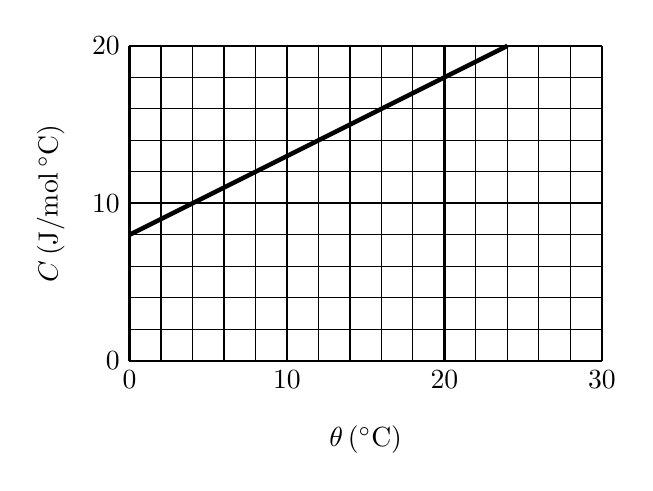
\begin{tikzpicture}[scale=2]
                \draw[step=0.2,black,thin]
                (0,0) grid (3,2);
                \draw[step=1,black,thick]
                    (0,0) grid (3,2);
                \draw
                    (1.5,-0.5) node {$\theta\,(\mathrm{^\circ C})$};
                \path
                    (0,0) node[below] {0} 
                    (1,0) node[below] {10} 
                    (2,0) node[below] {20} 
                    (3,0) node[below] {30};
                \draw
                    (-0.5,1) node[rotate=90] {$C\,(\mathrm{J/mol\,^\circ C})$};
                \path
                    (0,0) node[left] {0} 
                    (0,1) node[left] {10} 
                    (0,2) node[left] {20};
                \draw[ultra thick]
                    (0,0.8) -- (2.4,2);
            \end{tikzpicture}
        \end{figure}


        Qual o calor necessário para aumentar a temperatura do objeto de $10
        \,\mathrm{^\circ C}$ até $20\,\mathrm{^\circ C}$?
        \answer{$Q=\int_{\theta_i}^{\theta_f}C(\theta)\,d\theta=155\,\mathrm J$}

    \item
        (SOIF 2023) Considere um sistema físico de massa m cuja energia interna
        é dada pela expressão
        $$U=\frac{U_0}{e^{T_C/T}-1},$$
        em que $T_C$ representa uma temperatura característica do sistema, $U_0$
        é uma constante, e  $T$ a sua temperatura.
        \begin{enumerate}
            \item 
                Calcule a expressão do calor específico do material $c$ 
                \answer{
                    $c=\frac{dU}{dT}=
                    \frac{U_0T_Ce^{T_C/T}}{mT^2(e^{T_C/T}-1)^2}$
                }
            \item 
                Determine os valores limites quanto $T\ll T_C$ e $T\gg T_C$
                \answer{
                    $c\rightarrow\frac{U_0T_C}{mT^2}e^{-T_C/T},
                    \,c\rightarrow\frac{U_0}{mT_C}$
                }
            \item 
                Calcule o calor necessário para levar o sistema de $T_C$ até
                $2T_C$.
                \answer{$Q=\Delta U=\frac{U_0\sqrt e}{e-1}$}
        \end{enumerate}

    \item 
        (IPhO 1996) Uma peça de metal termicamente isolada é aquecida sob
        pressão atmosférica por uma corrente elétrica de forma que recebe
        energia elétrica a uma potência constante $P$. Isso leva ao aumento da
        temperatura absoluta $T$ do metal com o tempo $t$ como:
        $$T(t)=T_0\left(1+a\left(t-t_0\right)\right)^{1/4},$$
        onde $a$, $t_0$ e $T_0$ são constantes. Determine a capacidade térmica
        $C_p(T)$ do metal.
        \answer{$C=\frac{PT^3}{4aT_0^3}$}
\end{enumerate}
